\documentclass{article}

\usepackage[tmargin=2cm,rmargin=1in,lmargin=1in,margin=1in,bmargin=2cm,footskip=.2in]{geometry}
\usepackage[font=small,labelfont=bf]{caption}
\usepackage{graphicx}
\usepackage{listings}
\usepackage{multirow}
\usepackage{color}
\usepackage[T1]{fontenc}

\definecolor{codecomment}{rgb}{0,0.6,0}
\definecolor{codelinenumber}{rgb}{0.5,0.5,0.5}
\definecolor{codestring}{rgb}{0.58,0,0.82}
\definecolor{codebg}{rgb}{0.95, 0.95, 0.95}

\makeatletter
\def\@maketitle{
  \null
  \vskip 3cm
  \begin{center}%
    {\Large\bfseries \@title \par}
    \vskip 3em
    {\normalsize
      \lineskip .5em
      \begin{tabular}[t]{c}
        \@author
    \end{tabular}\par}
    \vskip 1cm
    {\normalsize \@date}
    \vskip 1cm
    \textbf{ADD GITHUB REPO LINK HERE}
  \end{center}%
  \par
  \vskip 1.5em}
\makeatother

% Attribution to David Carlisle (@david-carlisle) on TeX StackExchange
% https://tex.stackexchange.com/questions/618849/how-to-create-subsubsubsection
\makeatletter
\renewcommand\paragraph{\@startsection{paragraph}{4}{\z@}%
                                     {-3.25ex\@plus -1ex \@minus -.2ex}%
                                     {1.5ex \@plus .2ex}%
                                     {\normalfont\normalsize\bfseries}}
\setcounter{secnumdepth}{4}
\makeatother

\lstset{
  backgroundcolor=\color{codebg},
  basicstyle=\ttfamily\footnotesize,
  breakatwhitespace=true,
  breaklines=true,
  captionpos=b,
  commentstyle=\color{codecomment},
  escapeinside={\%*}{*)},
  extendedchars=true,
  frame=lines,
  keepspaces=true,
  keywordstyle=\color{blue},
  numbers=left,
  numbersep=10pt,
  numberstyle=\tiny\color{codelinenumber},
  rulecolor=\color{black},
  showspaces=false,
  showstringspaces=false,
  showtabs=false,
  stepnumber=1,
  stringstyle=\color{codestring},
  tabsize=4,
  captionpos=top
}



\usepackage{listings}
\usepackage{hyperref}

\graphicspath{{assets/}}

\title{Podcast Management System "FLOSScaster" \\
	\begin{large}
	WP-Seminar "Quelloffene Software in der modernen Informatik" Projekt
	\end{large} \\
  \begin{normalsize}
    Frankfurt University of Applied Sciences
  \end{normalsize}
}

% TODO sort alph. when all names are included
\author{
  dkar001 \\
  \texttt{-}
  \and
  Lepore, Dominik \\
  \texttt{dominik.lepore@stud.fra-uas.de}
  \and
  Fluegel, Dwipa \\
  \texttt{dwipa.fluegel@stud.fra-uas.de}
  \and
  Michael Filatoff \\
  \texttt{michael.filatoff@stud.fra-uas.de}
  \and
  Brychcy, Patryk \\
  \texttt{patryk.brychcy@stud.fra-uas.de}
  \and
  Gavrilov, Sascha \\
  \texttt{sascha.gavrilov@stud.fra-uas.de}
  \and
  Zimmermann, Alwin \\
  \texttt{alwin.zimmermann@stud.fra-uas.de}
  \and
  Zundel, Benedikt \\
  \texttt{benedikt.zundel@stud.fra-uas.de}
}

\date{Friday, 2025-05-23}

\begin{document}

\maketitle

\newpage

\tableofcontents
\listoffigures
\lstlistoflistings

\newpage

\section{Projektmanagement mit Scrum \& GitHub Projects \small{(Deniz Karaman)}}
Um unseren Entwicklungsprozess agil zu strukturieren, haben wir Scrum mithilfe von GitHub Projects implementiert. Dabei haben wir uns an klassischen Scrum-Prinzipien orientiert und diese wie üblich an unsere Teamgröße und die Projektanforderungen angepasst. Jede Story wird dabei als Issue angelegt.

Zunächst haben wir in unseren Issues sowohl Labels als auch Milestones definiert, um einen schnellen Überblick zu gewährleisten und einzelne Issues entsprechend ihrer Zuordnung hervorzuheben. Da wir unsere Stories im Team abgestimmt und deren Komplexität berücksichtigt haben, gelten die Definition of Done (DoD) sowie die Bewertung als feststehend.

Folgende Labels haben wir definiert: \textit{backend}, \textit{bug}, \textit{documentation}, \textit{enhancement}, \textit{epic}, \textit{frontend}, \textit{story}, \textit{testing}. Zusätzlich zu unseren Labels benötigen wir unterschiedliche Status, für die wir folgende verwenden: \textit{Todo}, \textit{In} \textit{Progress}, \textit{Needs} \textit{Review}, \textit{Done}, \textit{Canceled}.

Durch die Nutzung von Custom Fields vom Typ Iteration können wir unsere Sprints zeitlich organisieren und in wöchentlichen Zyklen abbilden. Bei der Sprintplanung in unseren Meetings haben wir zudem die Möglichkeit, sowohl die Story Points als auch die Priorität (\textit{Low}, \textit{Medium}, \textit{High}, \textit{Critical}) über Custom Fields abzubilden.

Nach Abschluss eines Sprints könnte eine formale Retrospektive stattfinden. Da wir jedoch durch unsere flexiblen Arbeitszeiten agil bleiben und unsere Sprints fortlaufend anpassen wollten, haben wir auf eine feste Retrospektive verzichtet.

\subsection{Darstellung Boards}
\begin{figure}[h]
  \caption{Screenshot der GitHub Projects Ansicht des Backlogs}
  \centering
  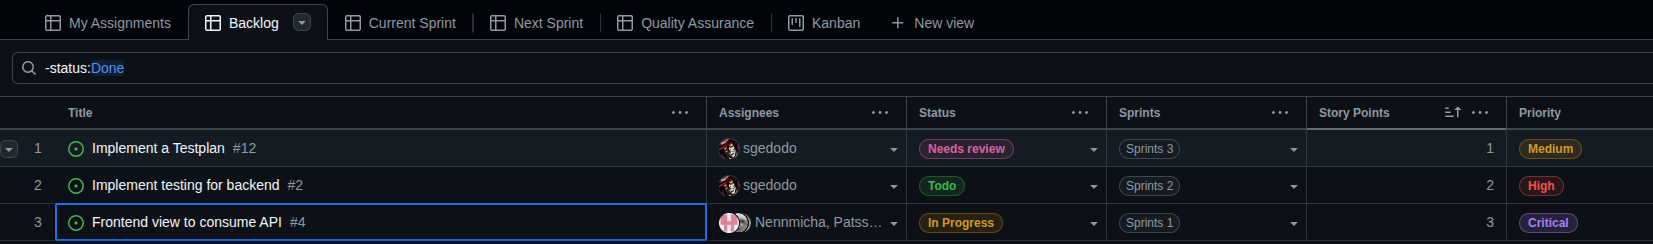
\includegraphics[width=\textwidth]{backlog.png}
\end{figure}

Um die Übersichtlichkeit weiter zu erhöhen, haben wir für jede Board-Ansicht vordefinierte Filter konfiguriert.

So erhält jede Ansicht genau die Issues, die für den jeweiligen Arbeitsschritt relevant sind, und das Team behält jederzeit den passenden Fokus.

\begin{figure}[h]
  \caption{Screenshot der GitHub Projects Ansicht der Quality Assurance}
  \centering
  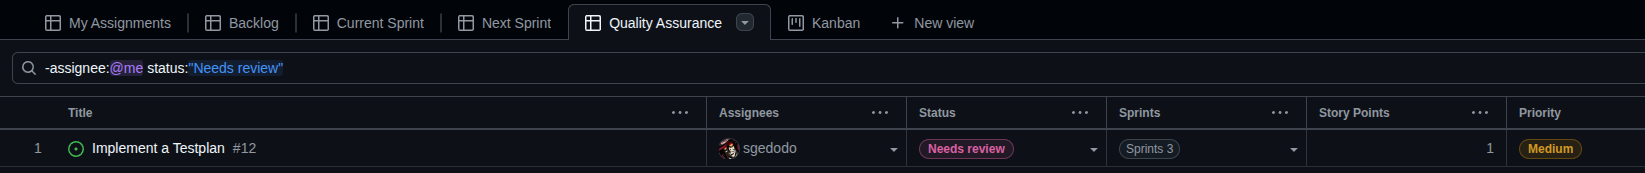
\includegraphics[width=\textwidth]{quality_assurance.png}
\end{figure}

\begin{itemize}
  \item \textbf{Backlog}: Alle geplanten User Stories und Tasks
  \item \textbf{Current Sprint}: Die aktuell bearbeiteten Items
  \item \textbf{Next Sprint}: Vorgemerkte Stories für den nächsten Sprint
  \item \textbf{Quality Assurance}: Abgenommene Features in der Testphase
  \item \textbf{Done}: Abgeschlossene Stories
\end{itemize}

Jeder Eintrag auf dem Board ist als GitHub Issue angelegt und hat folgende Felder

\begin{enumerate}
  \item Story Points (zur Aufwandsschätzung in Fibonacci)
  \item Priority-Labels (\textit{Low}, \textit{Medium}, \textit{High}, \textit{Critical})
  \item Sprint-Labels (z. B. \textit{Sprint1}, \textit{Sprint2}, etc.)
  \item Status-Labels (\textit{Todo}, \textit{In Progress}, \textit{Needs review}, \textit{Done}, \textit{Canceled})
\end{enumerate}

\begin{figure}[h]
  \caption{Screenshot der GitHub Ansicht einer Story}
  \centering
  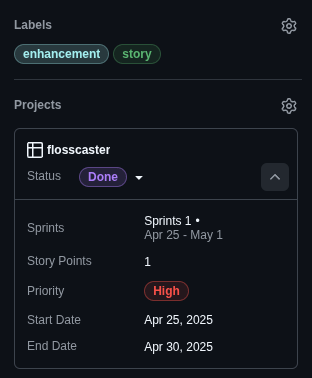
\includegraphics[width=.3\textwidth]{overview.png}
\end{figure}

Durch diese enge Verzahnung von Issue-Tracking, Code-Repositories und agilen Meetings erreichen wir eine hohe Transparenz, schnelle Feedback-Zyklen und eine stetige Verbesserung unseres Workflows.

\section{Static Code-Analyse (Deniz Karaman)}
Für die statische Code‐Analyse im Backend haben wir die integrierte Inspektions-Engine von \texttt{PyCharm (JetBrains)} eingesetzt. Dabei konnten wir verschiedene Probleme im Code identifizieren. Zu den häufigsten Befunden gehörten unter anderem:

\begin{itemize}
  \item Unresolved references
  \item Method is not declared static
  \item PEP 8 naming convention violation 
  \item Redundant parentheses
  \item Shadowing built-in names
  \item Shadowing names from outer scopes
  \item Using equality operators to compare with None
\end{itemize}

Dank dieser statischen Prüfung konnten wir gezielt Code-Stellen verbessern – etwa fehlende Imports ergänzen, Methoden korrekt deklarieren und PEP 8-konforme Bezeichner verwenden. Durch die frühzeitige Erkennung und Behebung dieser Probleme haben wir die Qualität, Wartbarkeit und Lesbarkeit unserer Anwendung weiter gesteigert.

\section{Mockup-Design und Gestaltung \small{(Patryk Brychcy \& Michel Filatoff)}}
\subsection{Planung}
In einem ersten Planungsschritt entschieden wir gemeinsam, dass die gesamte Funktionalität auf einer einzigen HTML-Webseite umgesetzt werden soll. Die Seite sollte so einfach, übersichtlich und benutzerfreundlich wie möglich gestaltet werden.

Daraufhin habe wir mithilfe des Online-Design-Tools \textit{Figma} das erste Mockup erstellt. Dieses visuelle Konzept stellt eine minimalistische und funktionale Benutzeroberfläche dar, die sich auf die wesentlichen Elemente konzentriert.

\begin{figure}[h]
  \caption{Figma Design der Landingpage}
  \centering
  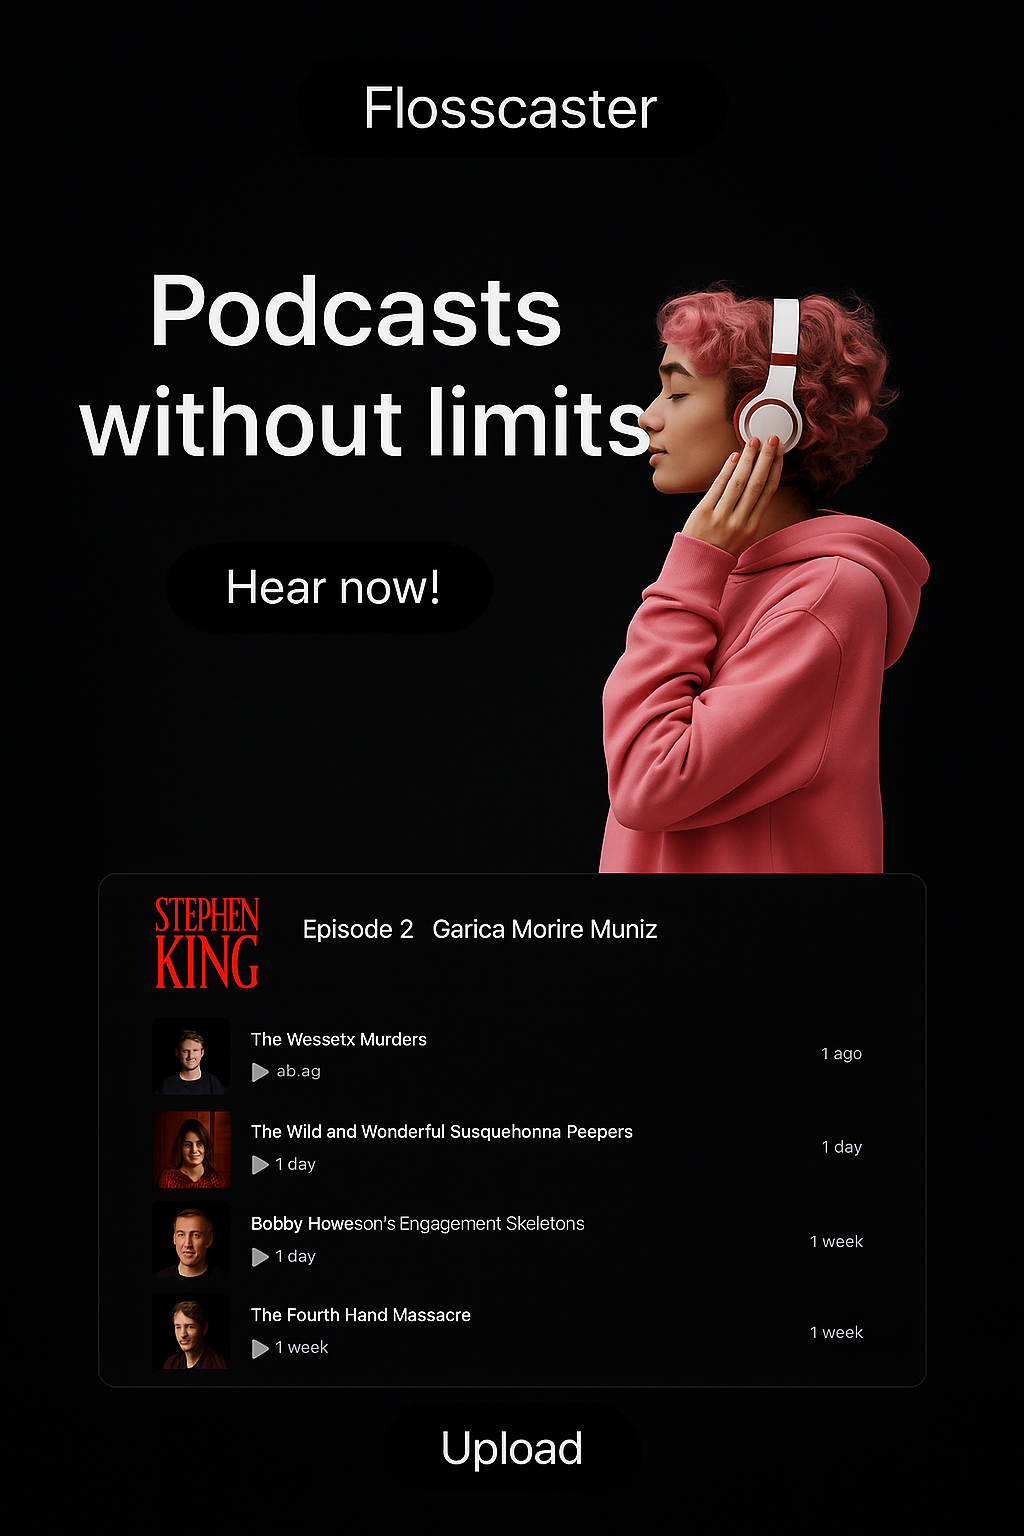
\includegraphics[width=0.4\textwidth]{flosscaster1.png}
\end{figure}

\begin{figure}[h]
  \caption{Figam Design des Upload-Dialogs}
  \centering
  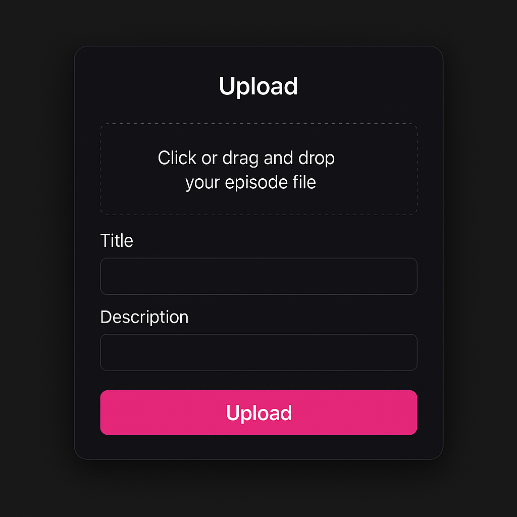
\includegraphics[width=0.3\textwidth]{flosscaster2.png}
\end{figure}

Die Webseite wurde dabei so angelegt, dass es flexibel ausbaufähig bleibt, das \textit{Flosscaster}-Logo oben am Rand ist eine Navigationsleiste (\texttt{Navbar),} wo man auch in der Zukunft eine Benutzerverwaltung integrieren könnte.

Die Webseite soll den Nutzern folgendes ermöglichen:

\begin{itemize}
  \item Neue Podcast-Folgen in einem klar strukturierten Umfeld zu entdecken
  \item Eigene Podcasts hochzuladen über einen gut sichtbaren Upload-Button
  \item Intuitives Fenster für das Hochladen der Podcasts
\end{itemize}

\subsection{Aufbau und Layout}
\subsubsection{Hero-Sektion}
\begin{itemize}
  \item \textbf{Titel \& Claim}: „Podcasts without limits“ – in großer, fetter Schrift als Blickfang
  \item \textbf{Call-to-Action-Button}: Handlungsaufforderung als „Hear now“-Button direkt unter dem Text
  \item \textbf{Visuelles Element}: Ein Porträt einer Person mit Kopfhörern vor einem Pink-Gradient-Hintergrund, das für Emotionalität und Wiedererkennbarkeit sorgt
\end{itemize}

\subsubsection{Latest Episodes}
\begin{itemize}
  \item \textbf{Überschrift}: Deutlich hervorgehoben mit weißer, serifenloser Schrift
  \item \textbf{Upload-Button}: Oben rechts platziert, damit der User mit Leichtigkeit neue Podcasts hochladen kann.
  \item \textbf{Episoden-Karten}:
  \begin{itemize}
    \item Abgerundete Ecken und leicht abgesetzter Hintergrund (dunkles Anthrazit)
  \end{itemize}
  \item \textbf{Jede Karte enthält}:
  \begin{itemize}
    \item Titel der Episode in fetter, weißer Schrift
    \item Kurzbeschreibung in grauer Schrift (mehrzeilig, lesefreundlich)
    \item Audioplayer mit Play/Pause-Funktion, Lautstärkeregelung und Fortschrittsbalken
  \end{itemize}
\end{itemize}

\subsubsection{Updates}
Das Design wurde im Laufe der Tests in mehreren Punkten überarbeitet.

\begin{itemize}
  \item Die Buttons sind pink und der Hero-Bereich hat pinke Akzente
  \item Die Liste mit Podcasts wurde nach unten versetzt und der „Hear Now“-Button scrollt nach unten auf die Podcasts-Liste
  \item Das Upload-Fenster wurde überarbeitet.
\end{itemize}

\subsubsection{Umsetzung \& Endergebnis}
Durch gezielte Anpassungen in den CSS-Dateien konnte das Design final umgesetzt werden. Das Ergebnis ist eine schlichte, funktionale und optisch ansprechende Webseite.

\begin{figure}[h]
  \caption{Implementiertes Design der Landingpage}
  \centering
  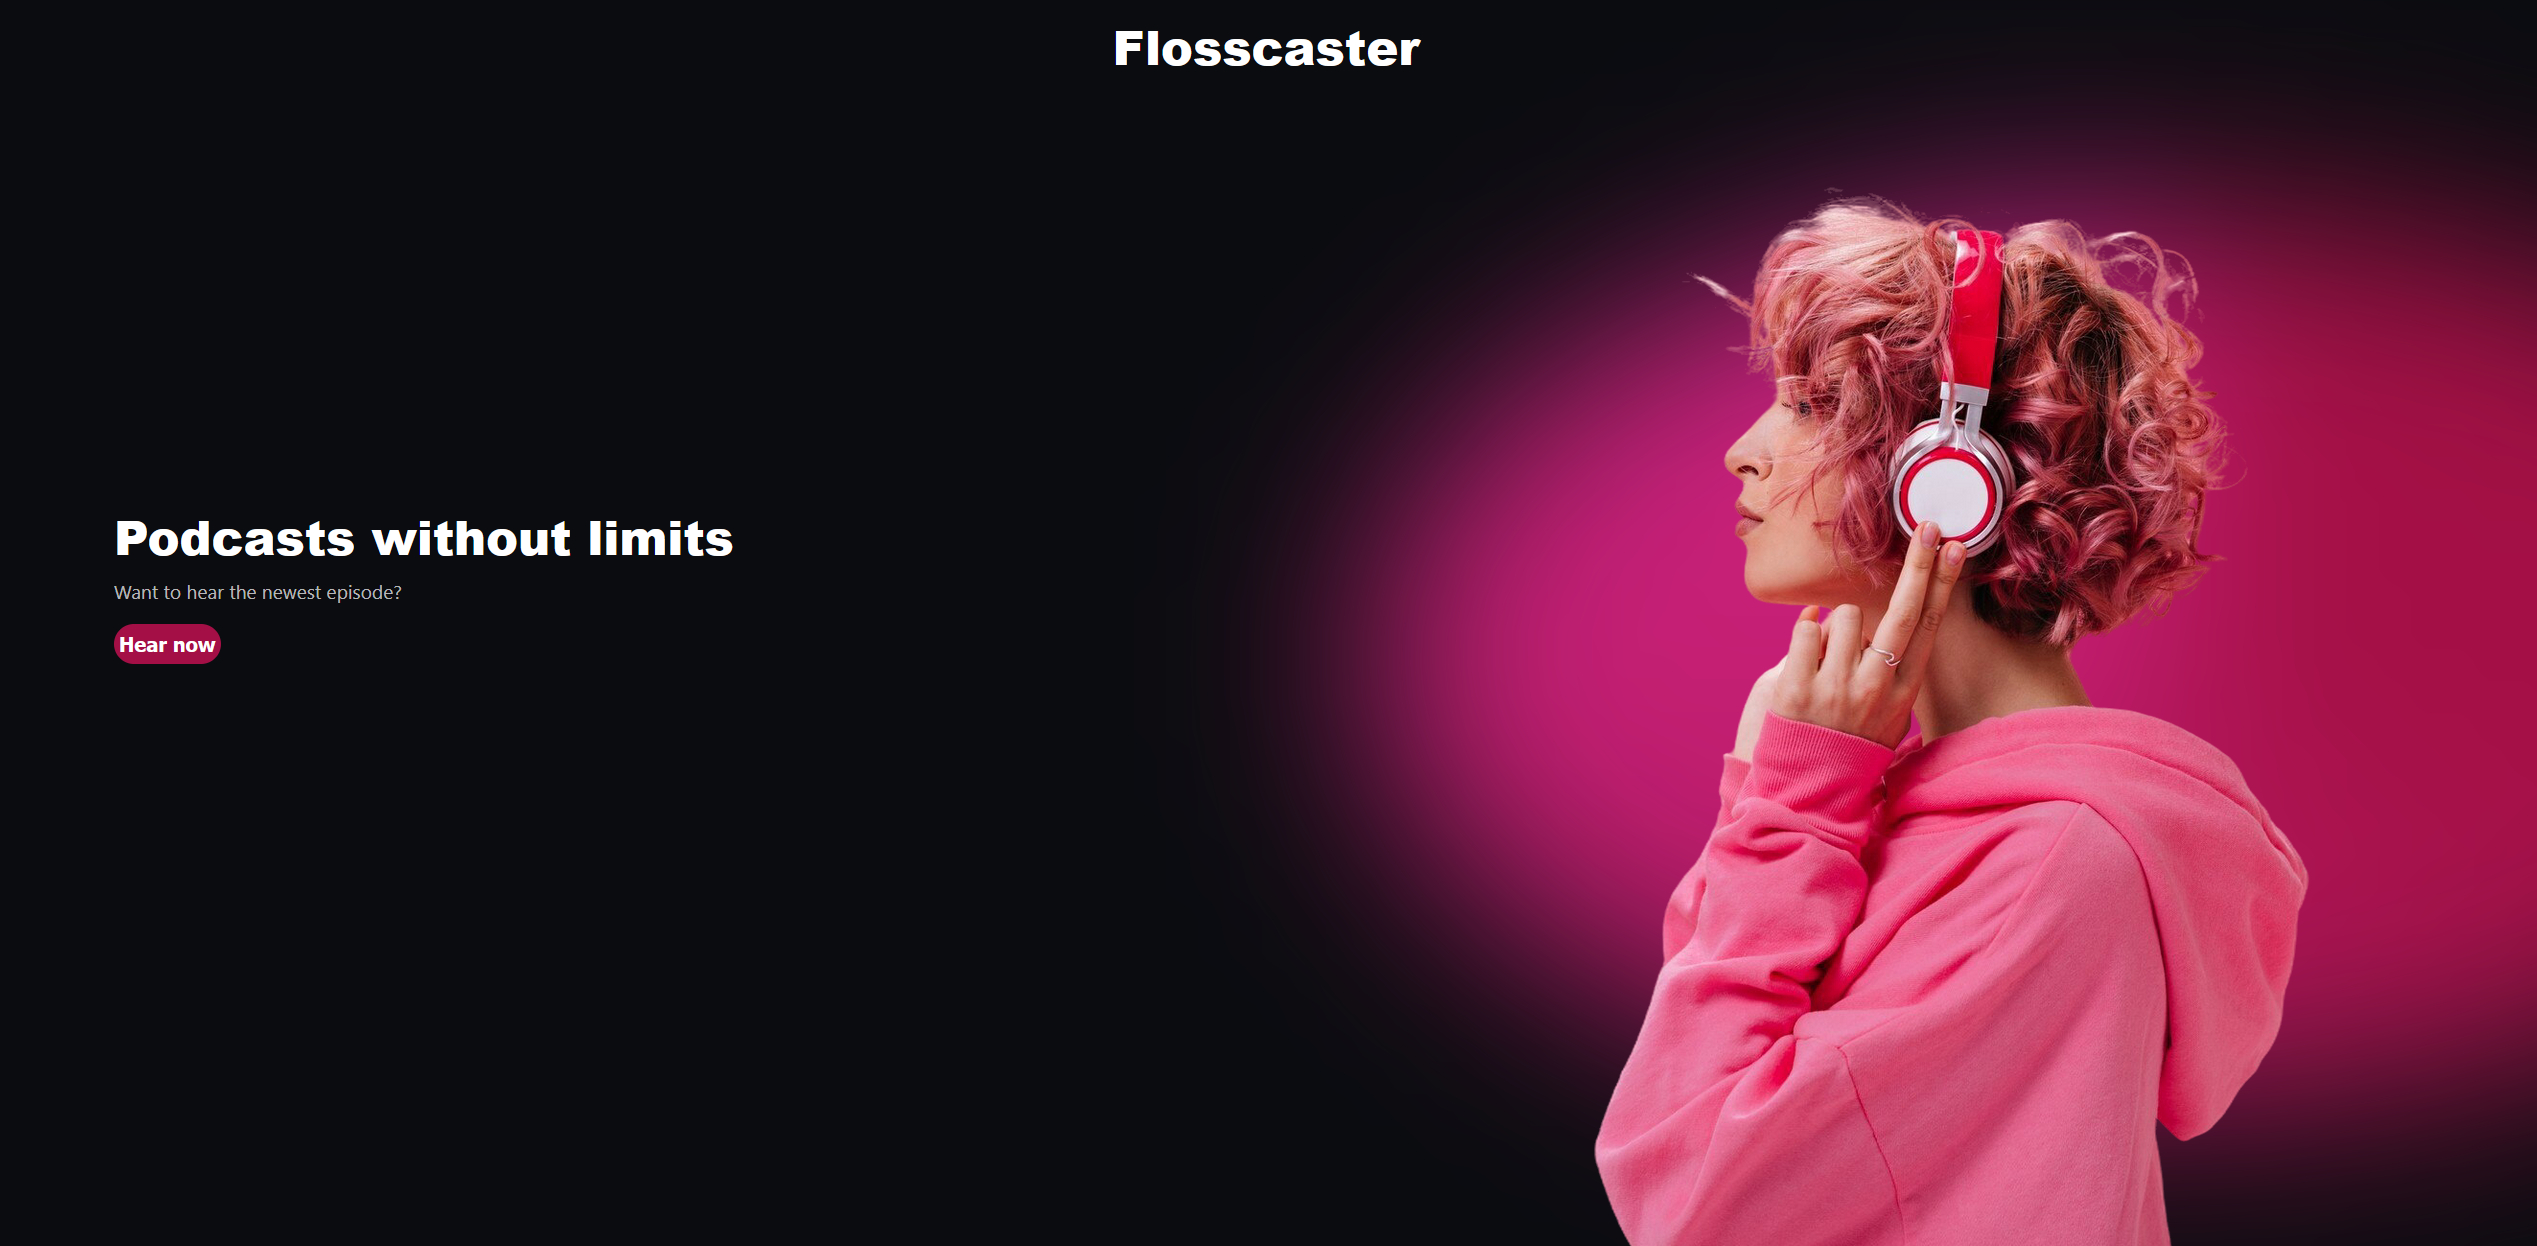
\includegraphics[width=0.7\textwidth]{flosscaster3.png}
\end{figure}

\subsubsection{Verwendete Designprinzipien}

\begin{itemize}
  \item \textbf{Dark Mode} mit pinken Akzenten
  \item \textbf{Akzentfarbe Pink} (\texttt{\#D81B60}) für interaktive Elemente
  \item \textbf{Weißer Text} für Überschriften zur klaren Strukturierung
  \item \textbf{Grauer Text} für Fließtexte und sekundäre Informationen
  \item \textbf{Abgerundete Buttons \& Karten}
  \item \textbf{Intuitive Buttons} mit klarer Beschriftung
  \item \textbf{Font Smoothing}: antialiased für bessere Textdarstellung
  \item \textbf{Smoothed Interface} für visuelle Harmonie und Benutzerfreundlichkeit
  \item \textbf{Hover-Effekte} für die Buttons und das Navbar
  \item \textbf{Verzicht auf überflüssige Elemente}
\end{itemize}

\begin{figure}[h]
  \caption{Implementiertes Design der Podcast-Episoden}
  \centering
  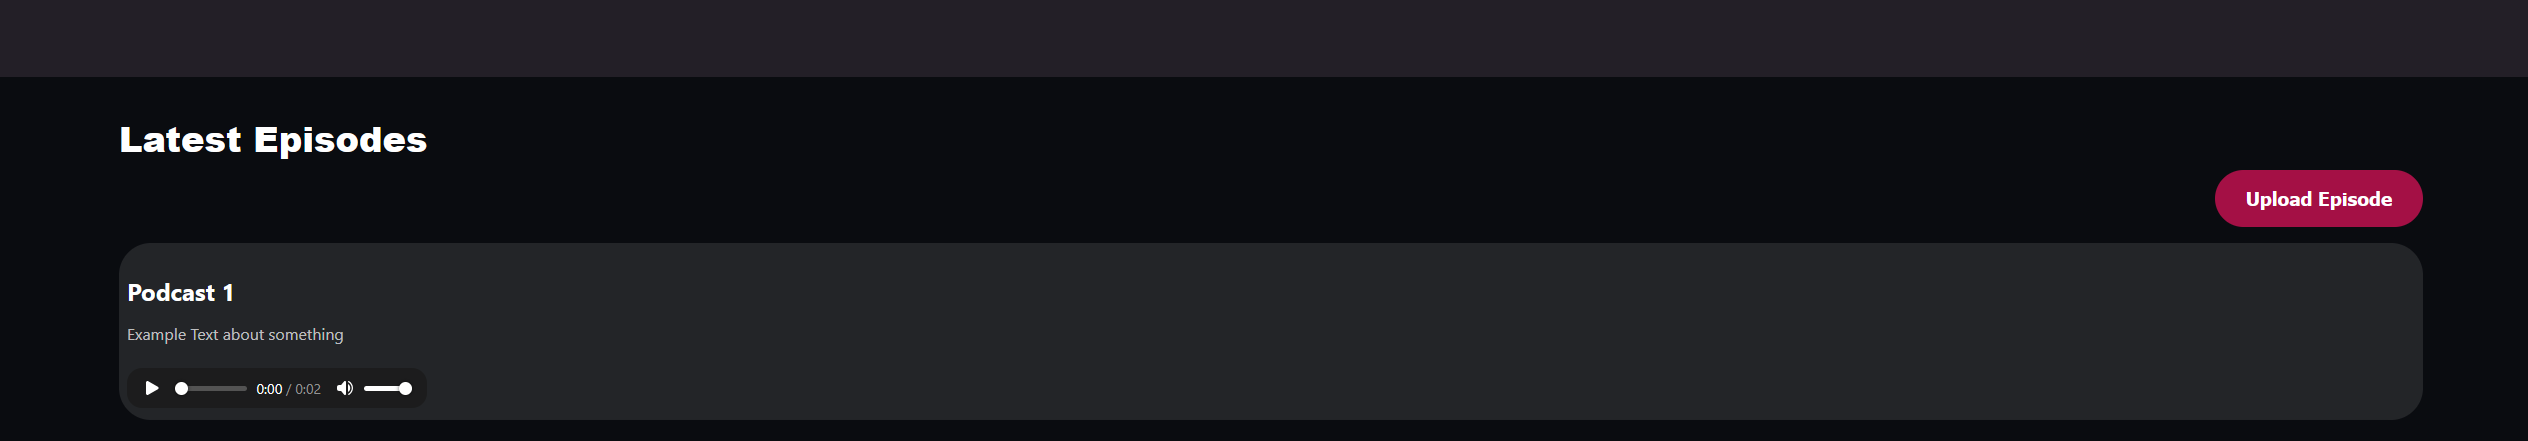
\includegraphics[width=0.9\textwidth]{flosscaster4.png}
\end{figure}

\section{Technische Dokumentation}
\subsection{Frontend \small{(Michael Filatoff)}}
Das Frontend haben wir mit den folgenden drei Kerntechnologien erstellt. \texttt{HTML5} wurde für die Struktur verwendet, \texttt{CSS3} für das Styling und JavaScript für die Funktionalität. Grundlegend wurde die gesamte UI mit der populären JavaScript-Bibliothek \texttt{React} zur Erstellung verwendet. Da \texttt{React} den Entwicklungsprozess vereinfacht und strukturiert, basiert unsere Architektur auf der \textit{Komponenten basierte Architektur}, die es uns ermöglicht, wiederverwendbare UI-Komponente zu erstellen. Außerdem benutzten wir die Zustandsmanagementfunktionen, welche Funktionen wie \texttt{useState}, \texttt{useEffect}, etc... anbieten. Diese helfen, die Daten, welche wir von dem API-Endpoint aus dem Backend erhalten, zu speichern und zu verwenden.

\subsubsection{Komponenten}
Grundlegend sind die Komponenten mit einer \texttt{.jsx} und \texttt{.module.css} Datei ausgestattet. Das \texttt{JSX} ist eine Erweiterung von JavaScript, die es ermöglicht, HTML Code innerhalb von JavaScript-Dateien zu schreiben. Die CSS Struktur basiert auf das Modul-Prinzip, wo Klassen und Namen nur lokal und nicht global gültig sind. Diese sind erst mit dem Import der CSS-Datei gültig.

\paragraph{Bar}
Die Bar-Komponente dient als Balken der für die Trennung zwischen der HeroSection und der Podcastlist-Section fungiert.

\paragraph{Hero}
Die Hero-Komponente enthält eine Sektion die aus einem Header, Paragraphen und einen Button besteht. Für den Button wurde der HTML tag \texttt{input} mit dem Typ \texttt{button} verwendet, welcher die \texttt{Id} von dem \texttt{div} aus der Datei \texttt{podcastLists} entnimmt und dorthin navigiert. Zusätzlich in der Hero-Sektion ist ein großes Bild, das sogenannte Hero-Bild.

\begin{lstlisting}[label=lst:frontend-hero-image, language=html, caption=Implementation des Hero-Bilds]
<img className={styles.mainPicture} src="./assets/hero_picture.png" alt="Hero Section"/>
\end{lstlisting}

\paragraph{Navbar}
Die Navbar-Komponente beinhaltet ausschließlich ein HTML tag \texttt{a}, welcher als Titel der Website dient. Zusätzlich besitzt der tag den \texttt{href} (hypertext reference), welcher leer ist und nach jedem Klicken wird man wieder zurück an den Start der Website navigiert.

\begin{lstlisting}[label=lst:frontend-navbar, language=html, caption=Implementation der Navbar]
<a href="/" className={styles.mainHeader}>
  Flosscaster
</a>
\end{lstlisting}

\paragraph{Podcast List}
Die \texttt{Podcastlist}-Komponente ist dafür zuständig, eine Liste von Podcast-Episoden anzuzeigen und dem User die Möglichkeit zu geben, neue Episoden hochzuladen. Diese interagiert mit dem Backend, um Episoden abzurufen und neue Episoden zu speichern.

Folgende Funktionalitäten sind in der \textit{podcast list} enthalten:

\begin{itemize}
  \item \textbf{State Management}: Die Komponente verwendet React Hooks, wie. z.B \texttt{useState} oder \texttt{useEffect,} um den Zustand von Variablen zu verwalten und speichern.
  \item \textbf{Wichtige Funktionen}:
  \begin{itemize}
    \item \texttt{handleOpen()} / \texttt{handleClose()}: Funktionen, um das Upload-Formular ein- bzw. auszublenden.
    \item \texttt{handleSumbit(event)}: Wird beim Absenden des Upload-Formulars ausgelöst. Bereitet die Daten als \texttt{FormData} vor und sendet die per POST-Methode an den Backend-Endpunkt \texttt{/api/create}. Zum Schluss setzt er die Formularfelder zurück aktualisiert die Episodenliste bei Erfolg.
    \item \texttt{WorkspaceEpisodes()}: Ruft die Liste der Episoden vom Backend-Endpunkt \texttt{/api/list} ab und aktualisiert den \texttt{episodes}-Zustand mit den empfangenen Daten.
  \end{itemize}
\item \textbf{Aufbau der UI}: Eine Überschrift, einen Button der bedingt das UploadFormular anzeigen lässt. Dieser besteht aus drei Eingabefeldern mit Titel, Beschreibung und eine Audio Datei, die mit einem \textit{Submit Button} versendet wird.
\item \textbf{Aufbau der Podcast-Episoden UI}: Jede Episode wird als \textit{Karte} \texttt{podcastCard} dargestellt. Die zeigt den Titel, die Beschreibung und die abspielbare Audio Datei, vom Backend-Endpunkt \texttt{/api/getupload} streamt.
\item \textbf{Backend-Kommunikation}: Die Basis-URL für Backend-Anfragen wird über die Umgebungsvariable \texttt{REACT\_APP\_BACKEND\_HOST} konfiguriert oder verwendet standardmäßig \texttt{localhost.} Die Kommunikation erfolgt über den Port 1111.
\end{itemize}

\paragraph{App}
Die App-Komponente ist die Hauptkomponente. Sie definiert die grundlegende Struktur und das Layout der Webseite, indem sie verschiedene wiederverwendbare Unterkomponenten importiert und anordnet.

\subsubsection{Styling \small{(Sascha Gav)}}
\paragraph{\texttt{module.css}}
Die Verwendung von \texttt{.module.css} ist eine spezielle Methode, um sicherzustellen, dass die in dieser Datei definierten Stile nur auf diesem spezifischen Teil der Webseite angewendet werden und nicht versehentlich das Aussehen anderer Teile ändern. \texttt{styles} wird zu einem Objekt, das wir verwenden können, um diese spezifischen Stile anzuwenden.

\paragraph{\texttt{Index.css}}
\begin{sloppypar}
Die Datei \texttt{index.css} \textit{stylt} die gesamte Anwendung. Es wird einen dunklen Hintergrund gesetzt, Browser-Default-Abstände entfernt, sanftes Scroll-Verhalten bei \textit{In-Page-Links} aktiviert und ein globales \textit{Font-Fallback} (System- und Webfonts) definiert.
\end{sloppypar}

\paragraph{\texttt{Bar.module.css}}
Die Bar-Komponente \texttt{bar.module.css} fungiert in unserem Layout als Platzhalter und Trennelement zwischen dem Hero-Bereich und der Episoden-Liste. Ihre zentrale Klasse \texttt{.container} sorgt für einen halb-transparenten Hintergrund mit abgerundeten Ecken und genug Innenabstand.

\paragraph{\texttt{Navbar.module.css}}
Das Navbar-Modul \texttt{navbar.module.css} definiert das Styling der Navigationsleiste. Die Klasse \texttt{.navbar} richtet den Navigations-Container als Flexbox aus, zentriert alle enthaltenen Elemente horizontal und fügt oben einen Abstand von 30 Pixeln hinzu. Innerhalb dieses Containers übernimmt die Klasse \texttt{.mainHeader} die Gestaltung des Textes: große, fette Schrift in Weiß, keine Unterstreichung und ein sanfter Hover-Effekt, der die Schrift minimal vergrößert und den Hand-Cursor anzeigt, wenn man drauf zeigt.

\paragraph{\texttt{Hero.module.css}}
Im Hero-Modul \texttt{hero.module.css} wird der Fullscreen-Bereich an oberster Stelle umgesetzt. Die Klasse \texttt{.container} teilt den Bereich mittels Flexbox in einen linken Textbereich und einen rechten Bildbereich, beide in voller Browserhöhe. Der linke Bereich, also der Textbereich \texttt{.content} stapelt Überschrift, Untertitel und \textit{Hear now}-Button vertikal und zentriert sie auf der linken Seite, getrennt durch etwas Abstand zum Bild. Die Klassen \texttt{.mainHeader} und \texttt{.mainParagraph} legen Schriftart, Farben und Abstände für Titel und Untertitel fest. Der Button (\texttt{.heroButton}) erhält eine abgerundete Form, eine passende Farbe und ein sanftes Leuchten beim Hover. Das Bild selbst \texttt{.mainPicture} füllt seinen Bereich ohne Verzerrung aus. Dekorative Blur-Elemente im Hintergrund \texttt{.bottomBlur} erzeugen mit großer Fläche und Unschärfe einen modernen Tiefen­effekt.

\paragraph{\texttt{PodcastLists.module.css}}
\begin{sloppypar}
Schließlich beschreibt das \texttt{PodcastLists}-Modul \texttt{podcastLists.module.css} das Design der Episoden­übersicht und des zugehörigen Upload-Fensters. \texttt{.container} stapelt die einzelnen Podcast-Karten vertikal mit gleichmäßigem Abstand. 
Eine Überschrift im Stil der Klasse (\texttt{.mainHeader}) führt in die Listen-sektion ein. Jede Karte \texttt{.podcastCard} erhält durch halbtransparente Hinter­grund­farbe, Unschärfe („Glas-Effekt“), stark abgerundete Ecken und ein leichtes Skalieren bei Hover einen modernen Look. Innerhalb der Karten definieren die Klassen \texttt{.podcastTitle} und \texttt{.podcastDescription} die Schriftgrößen, die Schriftdicke und Abstände für Titel und Beschreibung. Der Audio-Player wird über eine eigene Klasse (audio) leicht abgerundet. 
Die Button Klasse \texttt{.showUploadBtn} gestaltet den \textit{Upload Episode}- Button, der das Upload-Fenster öffnet. Er ist in der Akzentfarbe der Webseite gestaltet und zeigt beim Hover einen Schatten und einen gedrückten Zustand beim Klick. 
Das Upload-Fenster selbst wird von der Klasse \texttt{.top} komplett im Viewport zentriert und erhält eine dunkle, fast deckende Hintergrundfarbe, passend zum Stil der restlichen Webseite, und feste Breiten- und Höhenbegrenzung. Die Textfelder im Fenster sind voll­breit, mit hohem Kontrast und ausreichendem Innen­abstand definiert. 
\end{sloppypar}

Abschließend \textit{stylt} \texttt{.submit} den \textit{Submit}-button in Akzentfarbe und \texttt{.close} positioniert das Schließ-Icon oben rechts im Uploadfenster.



\subsection{Backend \small{(Benedikt Zundel)}}
Als Kommunikationsschnittstelle mit dem Frontend haben wir uns für ein minimales restful \textit{application programming interface} (API) entschieden. Dafür haben wir unterliegend \texttt{flask}, insbesondere \texttt{flask-restful}, verwendet. Diese API legt die wesentlichen Endpunkte, die verwendet werden, um Podcast Episoden abzufragen und neue zu erstellen, frei. Zum sichern der Episoden verwenden wir eine dynamische Lösung, mit der Metadaten in einer leichtgewichtigen \texttt{SQLite} Datenbank abgelegt werden und die zugehörigen Audiodaten im Dateisystem gespeichert werden, mit einem Verweis auf den Pfad in der Datenbank. Rückwirkend wird entsprechend der Eintrag aus der Datenbank geholt und die Datei aus dem Dateisystem geladen.

\subsubsection{Modell}
Das unterliegende Modell, welches wir zur internen Darstellung der Podcast Episoden verwenden, besteht aus einer \texttt{dataclass} mit wenigen Feldern (vgl. Listing \ref{lst:episode_model}). Sie enthält eine \texttt{id}, welche eine eindeutige Identifikation des Elements darstellt, die Felder \texttt{title}, \texttt{description} und \texttt{date} in denen Metadaten der Episoden liegen und das Feld \texttt{filepath}, in dem der interne Pfad zur Audiodatei gesichert wird. Eine \texttt{dataclass} war für unsere Zwecke ausreichend, da es keine Anforderungen für komplexe Operationen gibt und somit keine Funktionen innerhalb der Klasse nötig sind, weshalb das Modell als reine Datenklasse implementiert werden kann.

\begin{lstlisting}[label=lst:episode_model, language=Python, caption=Implementation der Podcast-Episoden Klasse]
@dataclass
class Podcast:
    id: int
    title: str
    description: str
    date: str
    filepath: str
\end{lstlisting}

\subsubsection{Endpunkt: \texttt{/api/list}}
Der Endpunkt \texttt{/api/list} dient der Lieferung der vollständigen Auflistung aller Episoden und ist somit als \texttt{GET} Endpunkt definiert. Es wird kein Parameter im Aufruf erwartet. Intern wird bei einem Aufruf eine \texttt{SELECT *} SQL-Abfrage an die Datenbank gemacht. Das Ergebnis wird dann auf die Modellstruktur \textit{gecastet} und als \texttt{JSONArray} als Antwort zurückgeschickt.

\subsubsection{Endpunkt: \texttt{/api/create}}
Bei dem Endpunkt \texttt{/api/create} handelt es sich um einen \texttt{POST} Endpunkt, der für das Erstellen neuer Episoden verantwortlich ist. Bei einem Aufruf werden die Parameter \texttt{title} \& \texttt{description} erwartet, welche die Metadaten der zu erstellenden Episode repräsentieren, und die Audiodatei \texttt{audio}, welche dem \texttt{MP3}-Format entsprechen soll und im Dateisystem abgelegt wird. Die Datei wird auf die formalen Kriterien geprüft und bei Erfolg mit einer \texttt{UUID} versehen im Dateisystem gesichert um Kollisionen zu vermeiden. Anhand der übergebenen Metadaten und dem generierten Dateinamen wird ein Eintrag in die Datenbank angelegt. Sollten alle Operationen erfolgen, wird der neue Eintrag dem RSS-Feed angehangen und ein \textit{Toot} von dem verbundenen Mastodon Account gesendet. Die Antwort an die aufrufende Instanz besteht aus dem Erfolgscode \texttt{200} mit der internen \texttt{id} des erstellten Eintrags.

\subsubsection{Endpunkt: \texttt{/api/get\_upload/<path>}}
Dieser Endpunkt ist ein weiter \texttt{GET} Endpunkt, der dem Senden der Audiodatei aus dem Dateisystem dient. Als URL-Parameter wird der Dateiname der gewünschten Episode erwartet, der von dem Client aus dem \texttt{JSON}-Objekt gelesen wird. Mit Hilfe des Dateinamens und dem Wissen über das Verzeichnis, in dem die Audiodateien gespeichert sind, ließt die API die Datei aus dem Dateisystem und sendet diese als Antwort. Sollte die Datei nicht gefunden werden, Antwortet die API mit dem Fehlercode \texttt{404}.

\subsubsection{Endpunkt: \texttt{/rss}}
Zur Bereitstellung des RSS-Feeds wird der Endpunkt \texttt{/rss} verwendet, der, auf Basis der Umgebungsvariable, die den Pfad zur RSS-Feed Datei bestimmt, die Datei aus dem Dateisystem lädt und als Antwort sendet.

\subsubsection{Dokumentation}
Die Dokumentation der API (verfügbar unter dem \texttt{/apidocs} Endpunkt) ist im Code enthalten und wird durch \texttt{swagger} \cite{swagger} zur Laufzeit bereitgestellt. Listing \ref{lst:listdoc} ist ein Beispiel, welches die Dokumentation des \texttt{/api/list} Endpunkts bestimmt. Erkennbar ist, dass die Dokumentation in einem \texttt{YAML}-ähnlichen Format geschrieben wird. Dort lassen sich Schemata definieren (in diesem Fall die Struktur eines Podcast-Episoden Objekts), Rückgabecodes der API und Parameter, die für eine Abfrage relevant sind.

\begin{lstlisting}[label=lst:listdoc, caption=Dokumentationskommentar des \texttt{/api/list} Endpunkts]
class List(Resource):
    def get(self):
        """Returns all podcasts metadata in the database
        ---
        definitions:
            Podcast:
                type: object
                properties:
                    id:
                        type: integer
                    title:
                        type: string
                    description:
                        type: string
                    date:
                        type: string
        responses:
            200:
                description: A list containing all podcasts
                schema:
                    type: array
                    items:
                        $ref: "#/definitions/Podcast"
                examples:
                    [
                      {
                        'id': 1,
                        'title': '6-Sekunden Podcast',
                        'description': 'Wir hatten keine Zeit um ein Thema anzusprechen.',
                        'date': '2025-04-22T20:00:00Z',
                      },
                      {
                        'id': 2,
                        'title': '6-Sekunden Podcast: Part 2',
                        'description': 'Wir hatten wieder keine Zeit um ein Thema anzusprechen.',
                        'date': '2025-04-23T18:00:00Z',
                      }
                    ]
        """
...
\end{lstlisting}

\subsection{Dockerization \small{(Benedikt Zundel)}}
Um das Einrichten der Application auf einem Server zu vereinfachen, haben wir uns für die \textit{dockerisierung} (i.e. Befähigung mit Docker zu bauen) entschieden. Das Projekt lässt sich in zwei primäre Kategorien teilen: Das Frontend und das Backend. Beide Teile benötigen einen \texttt{Dockerfile}, der die jeweiligen Teile als isolierte \textit{Container} darstellt. Inhalt eines \texttt{Dockerfiles} ist eine Beschreibung des Bauvorgangs, der das Installieren von Abhängigkeiten, Kopieren von laufzeitrelevanten Dateien und Ausführen der Applikation beinhaltet. Um zu verhindern, dass mühselig zwei Container parallel gestartet werden müssen, haben wir \texttt{docker-compose} zur \textit{Container orchestrierung} eingesetzt. Mit \texttt{docker-compose} lassen sich multi-Container Anwendungen mit einem Kommando ausführen, indem ihr Verhalten in einer \texttt{YAML}-Datei definiert wird. Darin wird, im Falle dieses Projekts, beschrieben, welche Container gestartet, welche Ports offengelegt und welche Umgebungsvariablen verfügbar gemacht werden sollen. Anhand dieser Informationen werden die Container gebaut und isoliert gestartet. Eine direkte Kommunikation mit den Containern ist nur durch die freigegebenen Ports möglich, was zu einer erhöhten Sicherheit der Anwendung führt.

\subsection{Deployment \small{(Benedikt Zundel)}}
Didn't deploy yet, not much to say.

\subsection[RSS-Feed Generator \small{(Alwin Zimmermann)}]{RSS-Feed Generator \small{(Alwin Zimmermann)\footnote{Ich erkläre hiermit, dass ich bei der Erstellung dieses Projektes Unterstützung von ChatGPT, einem KI-gestützten Sprachmodell von OpenAI, in Anspruch genommen habe. Alle Inhalte wurden von mir überprüft und bearbeitet.}}}

\subsubsection{Ziel}
Das Ziel des Generators ist es, dass ein sogenannter Podcatcher den RSS Feed unseres Podcasts einlesen kann. Der RSS Feed muss hierfür von unserem Server als .XML (oder .rss) bereitgestellt werden. Bei einem RSS Feed gibt es einige wichtige Punkte zu beachten, die für den Aufbau eines syntaktisch richtigen Feeds beachtet werden müssen. Eine XML-Datei hat eine Baumstruktur, im Kopf stehen Infos wie: XML-Version, Encoding, RSS-Version.

\subsubsection{Struktur des RSS Feeds}
Nach dem Kopf steht die Channel-Sektion, in der der Channel die wichtigsten Werte erhält. Diese wären:
\begin{itemize}
    \item Titel
    \item Link zur Webseite
    \item Beschreibung
    \item Sprache
    \item Veröffentlichungsdatum
    \item Info, wann der Feed das letzte Mal erstellt/aktualisiert wurde
\end{itemize}

Ab diesem Bereich beginnen die Items, in denen die Infos über die neuen Podcast-Folgen hinzugefügt werden können. Jedes Item (jede Folge) hat:

\begin{itemize}
    \item Titel
    \item Link zur Episode
    \item Beschreibung
    \item Enclosure URL
    \item Veröffentlichungsdatum
\end{itemize}

Nach allen Items wird der Channel geschlossen und der RSS Feed beendet.

\subsubsection{Probleme}
Das Paket \texttt{feedparser} \cite{feedparser} hat leider das Problem, dass es die sogenannte Enclosure URL nicht parsen kann. Diese ist jedoch essenziell für den Podcatcher, um die Datei finden zu können (Issue: \#285 enclosure not parsed). Das Problem besteht nicht beim ersten Erstellen des Feeds, sondern erst beim Wiedereinlesen des Feeds. Eine mögliche Lösung hätte sein können, die Infos alle redundant zu speichern, jedoch habe ich diese Lösung schnell verworfen, da sie mit einem unverhältnismäßigen Aufwand verbunden wäre. Eine weitere Lösung könnte das Modul RSS in Ruby sein, jedoch wollte ich die Problematik in Python lösen, da die meisten Teile unseres Projekts bereits in Python geschrieben waren und ich selber bisher noch kein Ruby geschrieben habe.
Deshalb habe ich mich für das Paket \texttt{lxml} \cite{lxml} entschieden, welches ein generisches XML-Bearbeitungstool ist. Dieses ist zwar nicht speziell für RSS entworfen, sollte jedoch manuell in der Lage sein, den Feed entsprechend anzupassen.

\begin{lstlisting}[language=Python, caption=Feedparser Bug]
def load_existing_feed(self):
  """Laedt den bestehenden RSS-Feed, falls vorhanden."""
  if os.path.exists(self.feed_file_path):
      feed = feedparser.parse(self.feed_file_path)
      for entry in feed.entries:
          item = {
              'title': entry.title,
              'description': entry.description,
              'date': entry.published if 'published' in entry else datetime.now().isoformat(),
              'enclosure_url': entry.enclosure.href if 'enclosure' in entry else None,
              'enclosure_type': entry.enclosure.type if 'enclosure' in entry else None,
              'enclosure_length': entry.enclosure.length if 'enclosure' in entry else None
          }
          self.items.append(item)
          print(self)
\end{lstlisting}

\subsubsection{Das Script}
Das Script ist ein einfaches Python-Modul, das eine Funktion zum Hinzufügen von Podcasts in den Channel ermöglicht. Wichtig ist natürlich das Importieren der benötigten Python-Libraries.

\begin{lstlisting}[language=Python, caption=RSS-Feed Generator imports]
import os
import argparse
import datetime
import pytz
from lxml import etree
\end{lstlisting}

Als Input-Werte benötigt es lediglich:

\begin{itemize}
    \item einen Titel als String
    \item eine URL zu der Folge, die hinzugefügt werden möchte
    \item eine Beschreibung der Folge
\end{itemize}

Das Veröffentlichungsdatum wird als aktuelles Datum gewählt, da das Script automatisiert ausgeführt werden soll. Zudem wird der Audio-Typ auf MP3 festgelegt, da wir das FLAC-Format von Anfang an verworfen haben. Mithilfe von \texttt{lxml} wird nun ein neues \texttt{<item>} Objekt hinzugefügt mit den angegebenen Werten.

\begin{lstlisting}[language=Python, caption=Erstellen eines neuen Feed-Items]
# Erstelle ein neues Item
new_item = etree.Element('item')
etree.SubElement(new_item, 'title').text = title
etree.SubElement(new_item, 'description').text = description
etree.SubElement(new_item, 'pubDate').text = new_episode_pubDate
enclosure = etree.SubElement(new_item, 'enclosure')
enclosure.set('url', url)
enclosure.set('length', str(os.path.getsize(os.path.join(os.environ['UPLOAD_PATH'], os.path.basename(url)))))
enclosure.set('type', 'audio/mpeg')
\end{lstlisting}

Auch wird im Kopf das \texttt{lastBuildDate} auf den aktuellen Moment abgeändert. Zuletzt wird der neue XML-Feed dann in einen Ordner mit dem Namen \texttt{rss} abgespeichert und kann vom Server publiziert werden.

\begin{lstlisting}[language=Python, caption=Vollständige Funktion des RSS-Feed Generators]
def add_episode_to_podcast(title: str, url: str, description: str):
    # Verzeichnis und Dateiname
    directory = './rss'  # Aktuelles Verzeichnis mit dem Unterordner 'rss'
    filename = 'podcast.xml'  # Name der RSS-Datei

    # Vollstaendiger Pfad zur Datei
    file_path = os.path.join(directory, filename)

    # RSS-Feed laden
    with open(file_path, 'rb') as f:
        feed_content = f.read()

    # XML-Parser initialisieren
    root = etree.fromstring(feed_content)

    # Neue Episode hinzufuegen
    new_episode_pubDate = datetime.datetime.now(pytz.timezone('Europe/Berlin')).strftime('%a, %d %b %Y %H:%M:%S %z')

    # Erstelle ein neues Item
    new_item = etree.Element('item')
    etree.SubElement(new_item, 'title').text = title
    etree.SubElement(new_item, 'description').text = description
    etree.SubElement(new_item, 'pubDate').text = new_episode_pubDate
    enclosure = etree.SubElement(new_item, 'enclosure')
    enclosure.set('url', url)
    enclosure.set('type', 'audio/mpeg')

    # Fuege das neue Item zum Channel hinzu
    channel = root.find('channel')
    channel.append(new_item)

    # Aktualisiere lastBuildDate
    last_build_date = channel.find('lastBuildDate')
    last_build_date.text = datetime.datetime.now(pytz.timezone('Europe/Berlin')).strftime('%a, %d %b %Y %H:%M:%S %z')

    # Speichern des aktualisierten Feeds mit Zeilenumbruechen und Einrueckungen
    with open(file_path, 'wb') as f:
        f.write(etree.tostring(root, pretty_print=True, xml_declaration=True, encoding='UTF-8'))

    print(f'Die neue Episode "{title}" wurde erfolgreich zu {filename} hinzugefuegt.')
\end{lstlisting}

\subsection{Publikation auf einem Social Media Feed \small{(Dwipa Flügel)}}

\subsubsection{Ziel}
Das Ziel ist es auf mindestens einem Social Feed eine Ankündigung zu veröffentlichen, wenn eine neue Folge des Podcastes veröffentlicht wird. Vorteilhaft sollte diese Ankündigung dabei den Titel und die URL des Podcastes erhalten, damit die Zuhörer einen kleinen Überblick bekommen, als auch die möglichkeit bei Interesse direkt auf die neue Episode zuzugreifen über die URL.

\subsubsection{Auswahl und Entscheidung}
Es gibt eine große Auswahl an Social Media Plattformen auf denen man seine Anküdigungen veröffentlichen kann, haben uns aber im Kontext dieses FLOSS-Projektes für Mastodon entschieden. Mastodon ist eine quelloffene dezentralisierte Social Media Plattform und Teil des "Fediverse", einem Netzwerk von Servern die unabhängig voneinander operieren, welche das ActivityPub-Protokoll benutzen um miteinander zu kommunizieren. Hierbei können sich Benutzer frei aussuchen auf welcher Instanz sie ihren Account erstellen und trotzdem mit anderen Instanzen interagieren. In unserem Falle haben wir uns für die Hauptinstanz mastodon.social entschieden, da diese Leuten frei erlaubt einen Account herzustellen und nicht Einladungsbasierend ist, als auch die Benutzung von Bots nicht untersagt ist; da jede Instanz ihre eigenen Regeln besitzt, sollten diese auch befolgt werden.

\subsubsection{Zugriff auf die API}
Um mit unserer Mastodon-Instanz zu kommunizieren wird eine API-Verbindung gebraucht, da wir uns entschieden haben das Backend unseres Projektes in Python zu schreiben, bietet sich hierfür das \texttt{Mastodon.py} Modul an, welches "feature complete" ist. Zudem werden für die Benutzung der API Zugriffsdaten benötigt, welche generiert werden indem man auf der ausgewählten Instanz eine Anwendung registriert. Hier empfiehlt es sich dies über die UI der Instanz zu machen, welche unter \url{https://mastodon.social/settings/applications} gefunden werden kann.

\subsubsection{Probleme}
\begin{sloppypar}
Während meiner Forschung bezüglich der Moglichkeiten, wie man Podcast-Episoden automatisch ankündigt bin ich auf folgenden Blog-Post gestoßen: \url{https://c20d.blog/posts/2023/03/tootrss-utility/}. In diesem wurde ein Utility-Tool vorgestellt, bei dem neuhinzugefügte RSS-Items automatisch auf einen Mastodon-Account veröffentlicht werden. Dadurch das der Podcast auf einem RSS-Feed aufgebaut ist, hatte mich dieser Ansatz neugierig gemacht und ich hatte vor unsere eigene Version zu programmieren, welche auf SQLite aufgebaut war und nicht auf Amazons DynamoDB. Hier wurde das Paket feedparser benutzt, welches wie oben von Alwin beschrieben gewisse Probleme mit sich brachte, die sich im Verlauf der Entwicklung problematisch herausgestellt hat. Das Umgehen des RSS-Feedes hatte sich dadurch Problematisch gemacht, da das Paket beim parsing ein FeedParserDictionary ausgibt, wodurch sich das sortieren des RSS-Feedes auf das neuste Item mittels sorted() als nicht möglich erwieß. Ein Ansatz, der hier funktioniert hätte, welcher vom Autor des obig genannten Blog-Postes benutzt wurde, war das kreieren einer eigenen Klasse um gewisse Hilffunktionen aufzurufen, welchen ich als unverhältnissmäßigen Aufwand ansah. Nachdem ich mir einige Gedanken gemacht hatte und mir Alwins Code angeschaut habe, da er verantwortlich war für den RSS-Feed, musste ich mir eingestehen, dass das Design und die vorangehensweise sich als schlicht ineffizient herausgestellt hat. Dadurch das der Feed von uns verwaltet wird und die neuen Podcast-Episoden als neue Items in den Feed hinzufügt werden mit allen relevanten informationen für das veröffentlichen eines Tootes, hatte es weitaus mehr Sinn ergeben, ein Skript zu bauen, welches den gleichen Input benutzt und direkt danach aufgerufen wird.
\end{sloppypar}

Da wir hier mit Zugangsdaten arbeiten, sollte diese Informationen als Umgebungsvariablen gespeichert werden. Während des entwickeln hatte ich hierfür eine .env-Datei benutzt, welche ich natürlich in einer gitignore inkludiert hatte.

\begin{lstlisting}[language=Python, caption=Vollständige Funktion des \textit{Autotootings}]
def masttoot(title: str, url: str, description: str):
    """Publishes a new toot using the input, also sends a reply to the announcement with the description."""

    post_text = "The Flosscasters have released a new podcast episode: " + title + ". Check it out @ " + url

    #Mastodon-Instanz
    mastodon = Mastodon(
        client_id = os.getenv("MASTODON_CLIENT_KEY"),
        client_secret = os.getenv("MASTODON_CLIENT_SECRET"),
        access_token = os.getenv("MASTODON_ACCESS_TOKEN"),
        api_base_url = os.getenv("MASTODON_BASE_URL")
    )

    #Publish the toot and reply to it with the description
    to_reply = mastodon.status_post(post_text)
    mastodon.status_post(description, in_reply_to_id=to_reply.id)
\end{lstlisting}

\subsubsection{Gelerntes}

Ich habe leider verhältnismäßig viel Zeit investiert in ein Design, das sich nachträglich als ineffizient herausgestellt hat während der Entwicklung, wenn es eine weitaus einfachere Lösung gab. Im Kontext eines Uni-Projektes sollte dies etwas weniger Konsequenzen haben, aber im zukünftigen Kontext der Industrie sind das redundante Personalkosten. Da ich selber bei einem IT-Dienstleister arbeite, jedoch im 1st-Level Support, ist dies für mich eine wertvolle Lektion, da es schwer ist bei einem Kunden gewisse Stunden zu rechtfertigen, wenn diese nicht effektiv genutzt werden.

\newpage

\bibliographystyle{plain}
\bibliography{refs}

\end{document}
